%%%%%%%%%%%%%%%%%%%%%%%%%%%%%%%%%%%%%%%%%%%%%%%%%%%%%%%%%%%%%%%%%%% 
%                                                                 %
%                            CHAPTER                              %
%                                                                 %
%%%%%%%%%%%%%%%%%%%%%%%%%%%%%%%%%%%%%%%%%%%%%%%%%%%%%%%%%%%%%%%%%%% 

\chapter{Introduction}

Once per year, nearly a thousand volunteers travel to the Belgian coast to collect and categorize the shells that wash up on the beach. This data is collected by the Flemish Institute For The Sea (VLIZ) to study populations of marine mollusks and the impact of their environment (climate change, fishing, etc) on the population. The volunteers participating in this study are mostly enthusiasts, but also scientists and families with children. To ensure the quality of the data, most volunteers participate in a workshop prior to the activity. The counting of the shells is done by walking along the beach and logging every individual shell that is found. This is a very time-consuming process, and the volunteers are often not very experienced in counting, resulting in mistakes with all but the most common shells. When a volunteer finds a shell that they are not familiar with, they can contact a helpdesk to help them. The flowchart of the current process can be found in Figure \ref{fig:1_current_scenario}. 

\begin{figure}[h]
	\centering
	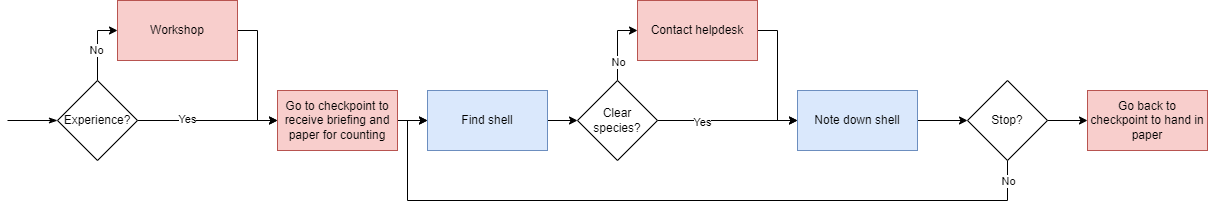
\includegraphics[width=1\textwidth]{chapter1/current_scenario}
	\captionsetup{belowskip=-\baselineskip}
	\caption{The current process of collecting data.}
	\label{fig:1_current_scenario}
	\setlength\belowcaptionskip{\baselineskip}
	\caption*{Marked blue is the volunteer's actions, and marked red are the parts that involve experts.}
\end{figure}

The fact that the project relies on volunteers to do most of the legwork, combined with experts having to man the checkpoints and the helpdesk, makes the project unscalable beyond having a single dedicated day each year. With over 5 million people
%https://www.kustportaal.be/nl/toerisme-en-recreatie#:~:text=De%20Belgische%20kust%20is%20de,in%20totaal%2027.723.420%20overnachtingen.
visiting the Belgian coast every year\cite{Kustportaal}, there is a lot of potential data to collect. To use this source of data, the process would have to be simplified and accessible to anyone visiting the beach at any time.

In this thesis, we will attempt to simplify the process of data collection so that it can be done by anyone, anywhere, at any time. We will do this with a counting network so that shells can be recognized in an image and counted automatically. This is already done on a smaller scale by VLIZ with Obsidentify, a mobile app and website where users can submit pictures of a single shell and get a result of what kind of shell it is. This is a useful tool, but taking a close-up picture of every single shell is again a very time-consuming process. 

As no dataset exists with large quantities of annotated pictures of beaches, we will have to work with a dataset of limited size to evaluate or train the neural network. After the successful completion of this thesis, the new ideal scenario for collecting data can be found in Figure \ref{fig:1_ideal_scenario}. Compared to the current process, found in Figure \ref{fig:1_current_scenario}, this new process nearly eliminates the experts' involvement and thus makes the process scalable.

\begin{figure}[h]
	\centering
	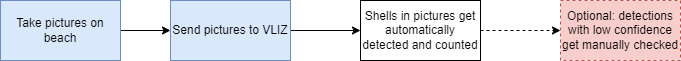
\includegraphics[width=0.8\textwidth]{chapter1/ideal_scenario}
	\caption{The new process of collecting data.}
	\label{fig:1_ideal_scenario}
\end{figure}

We will be testing if current counting networks are performant enough to recognize shells in beach images. We will do this by first introducing our dataset on which we will evaluate various methods. We will then discuss the state of the art in the field of object detection and counting, with a focus on few-shot learning. We then discuss how we will implement the models we studied. Next, the results and the limitations of the models are discussed. Finally, we will discuss future work that can be done to improve the model.